Observa los diseños en la figura \ref{fig:sucesion_cuadros01} y responde a las preguntas.

\begin{figure}[H]
    \centering
    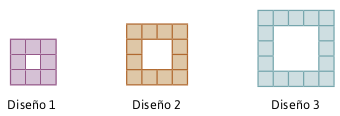
\includegraphics[width=.45\linewidth]{../images/sucesion_cuadros01}
    \caption{}
    \label{fig:sucesion_cuadros01}
\end{figure}

\begin{parts}
    \part ¿Cuántos cuadrados se añaden en cada diseño?

    \begin{solutionbox}{4em}
        4 cuadrados. El primero tiene 8, el segundo 12 y el tercero 16.
    \end{solutionbox}

    \part Completa la Tabla \ref{tab:3.5} y luego escribe una regla de recurrencia.

    \begin{table}[H]
        \rowcolors{3}{colorrds!10}{lightgray!10}
        \centering
        \caption{}
        \label{tab:3.5}
        \begin{tabular}{r|c|c|c|c|c|c|c|c|}
            \toprule
            \rowcolor{colorrds!80}
            {\bfseries\color{white}Posición del diseño} & {\bfseries\color{white}1} & {\bfseries\color{white}2} & {\bfseries\color{white}3} & {\bfseries\color{white}4} & {\bfseries\color{white}5} & {\bfseries\color{white}6} & {\bfseries\color{white}7} & {\bfseries\color{white}8} \\
            Número de cuadrados                         & \ifprintanswers8\fi       & \ifprintanswers12 \fi     & \ifprintanswers16\fi      & \ifprintanswers20\fi      & \ifprintanswers24\fi      & \ifprintanswers28\fi      & \ifprintanswers32\fi      & \ifprintanswers36\fi      \\ \cline{2-9}
            \bottomrule
        \end{tabular}
    \end{table}

    \begin{solutionbox}{8em}
        Los términos de la sucesión se pueden calcular con la siguiente regla:
        $8 + 4(n - 1) = 8 + 4n - 4 = 4 + 4n$
    \end{solutionbox}
     \renewcommand{\arraystretch}{1.4}
\end{parts}

